\documentclass{beamer}
%
% Choose how your presentation looks.
%
% For more themes, color themes and font themes, see:
% http://deic.uab.es/~iblanes/beamer_gallery/index_by_theme.html
%
\mode<presentation>
{
  \usetheme{Madrid}      % or try Darmstadt, Madrid, Warsaw, ...
  \usecolortheme{default} % or try albatross, beaver, crane, ...
  \usefonttheme{default}  % or try serif, structurebold, ...
  
  \makeatother
\setbeamertemplate{footline}
{
  \leavevmode%
  \hbox{%
  \begin{beamercolorbox}[wd=.5\paperwidth,ht=2.25ex,dp=1ex,center]{author in head/foot}%
    \usebeamerfont{author in head/foot}\insertshortauthor
  \end{beamercolorbox}%
  \begin{beamercolorbox}[wd=.4\paperwidth,ht=2.25ex,dp=1ex,center]{title in head/foot}%
    \usebeamerfont{title in head/foot}\insertshorttitle
  \end{beamercolorbox}%
  \begin{beamercolorbox}[wd=.1\paperwidth,ht=2.25ex,dp=1ex,center]{date in head/foot}%
    \insertframenumber{} / \inserttotalframenumber\hspace*{1ex}
  \end{beamercolorbox}}%
  \vskip0pt%
}
\makeatletter
  
  \setbeamertemplate{navigation symbols}{}
  \setbeamertemplate{caption}[numbered]
} 

\usepackage[english]{babel}
\usepackage[utf8x]{inputenc}
\usepackage{tikz}

\AtBeginSection[]{
  \begin{frame}
  \vfill
  \centering
  \begin{beamercolorbox}[sep=8pt,center,shadow=true,rounded=true]{title}
    \usebeamerfont{title}\insertsectionhead\par%
  \end{beamercolorbox}
  \vfill
  \end{frame}
}

\title[Waddle]{Waddle: \\ Waddington Epigenetic Landscapes}
\author{Felicia Burtscher, Lucas Ducrot, Madeleine Hall, Luis Torada}
\institute{MSc in Bioinformatics and Theoretical Systems Biology \\ Imperial College London}
\date{17th April 2018}

\begin{document}

\begin{frame}
  \titlepage
\end{frame}

%Uncomment these lines for an automatically generated outline.
\begin{frame}{Outline}
 \tableofcontents
\end{frame}

\section{Motivation, Introduction \& Workflow [FB]}

%I'M GOING TO LEAVE THESE SLIDES HERE FOR REFERENCE ON HOW TO INCLUDE MATHS AND FIGURES

\begin{frame}{Motivation}

\begin{figure}[b!]
\centering
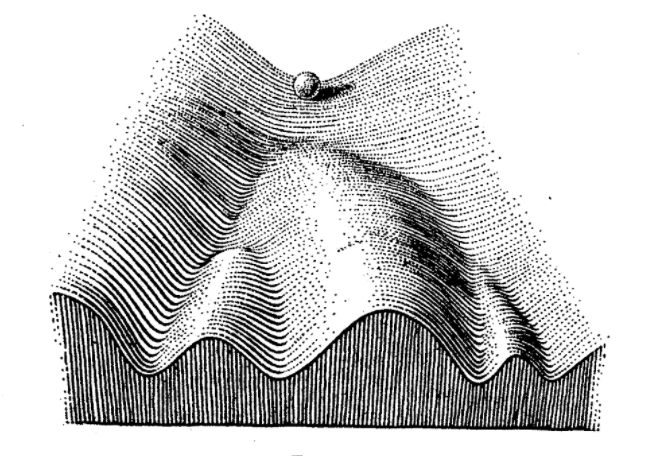
\includegraphics[width=4.6cm]{ball.PNG}
\caption{\textit{Part of an Epigenetic Landscape} (Waddington, 1940)}\label{ball}
\end{figure}
\textit{"The path followed by the ball […] corresponds to the developmental history of a particular part of the egg.
There is first an alternative, towards the right or the left. Along the former path, a second alternative is offered; along the path to the left, the main channel continues leftwards, but there is an alternative path which, however, can only be reached over a threshold"} (Waddington, 1940).
%The ball can be thought of as a cell, tracing a path corresponding to the expression of genes as it progresses through development. In 
%Figure \ref{ball}, there are four different destinations the ball could find itself in, corresponding to four different cell types a developing cell could end up as. Of course, in a given organism, the number of types of distinguished cell an undifferentiated cell could specialise to could be immense. 

\end{frame}

\begin{frame}{Introduction: Stochastic models}

From a stochastic system to an epigenetic landscape:
\begin{itemize}
\item Some stochastic systems can be expressed in terms of a potential.
\item Potential functions are similar to epigenetic landscapes.
\end{itemize}

\vfill
A general stochastic model is of the form: 
\begin{equation}\label{sde}
dX_{t} = f(X_{t}, t)dt + g(X_{t}, t) dW_{t}
\end{equation} 

and can be written as an ODE

\[  \frac{dX_{t}}{dt} = f(X_{t}, t)
\]

in the limit of low noise (high copy numbers).

\end{frame}

\begin{frame}{Introduction: Landscape formation}

Decomposition of the forcing vector $f(X; t)$:
\begin{equation}\label{decomp}
f(X; t) = -\nabla U(X; t) + f_U(X; t)
\end{equation}

where \( \nabla U(X; t) \) is the gradient of a potential, and \(f_U(X; t)\) is the remaining component, often referred to as the \textit{curl}.

\vfill
We call $U$ the \textit{quasi-potential} and it is analogous to the epigenetic landscape. $f_U$ is the remainder term, and fills out remaining dynamics. %(in some occasions, 
%MAYBE TOO VAGUE
%the curl is parallel to the contours). 

\end{frame}

\begin{frame}{Introduction: Define our goal}

\begin{itemize}
\item Literature review: Models like \textit{NetLand} (in Java) already available. 
\item Focus on visualisation by last year's group.
\end{itemize}

\vfill
Our focus:
\begin{itemize}
\item Methodology, less on visualisation
\item in Julia
\end{itemize}

\begin{block}{Goal}
Provide different tools and methods in Julia to 
(1) simulate and analyse the landscape and (2) visualise certain genes or gene combinations (after applying dimensionality reduction) given a single-cell data set.
\end{block}

\end{frame}

%\begin{frame}{Results}

%\end{frame}


\begin{frame}{Workflow}

\begin{figure}[h]
		\centering	
		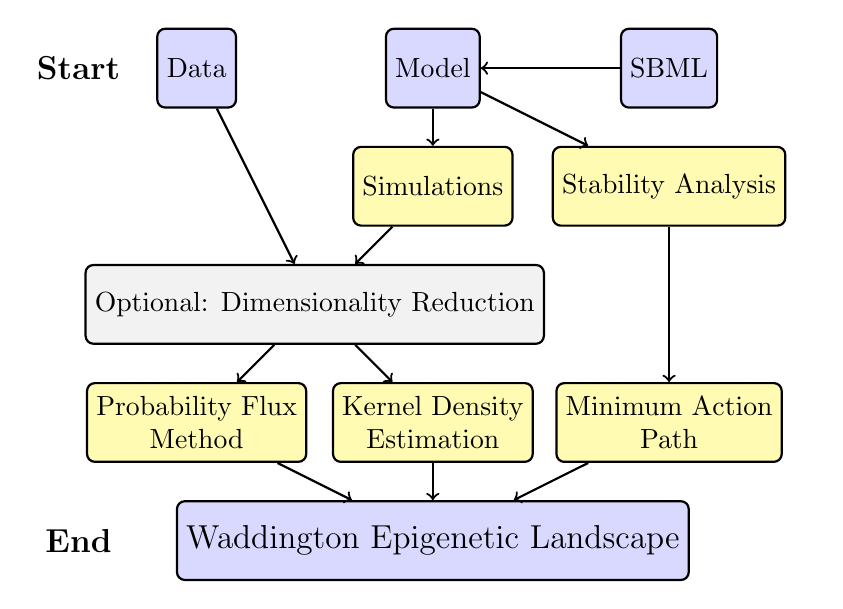
\begin{tikzpicture}[thick]
		%
		% Length scales for tikz diagram
		%
		\def\yunit{1.5} 
		\def\xunit{1.5}
		%
		% Aesthetic settings
		%
		\def\cornerrounding{0.1cm}
		%
		% Create grid of nodes		
		%
		\foreach \i in {1,...,35}
		{
			\pgfmathtruncatemacro{\y}{(\i - 1) / 7};
			\pgfmathtruncatemacro{\x}{\i - 7 * \y};
			\pgfmathtruncatemacro{\label}{\x + 7 * (4- \y)};
			\node[circle,minimum size=20]
			(\label) at (\xunit*\x,\yunit*\y) {};
		}
		%
		% 
		%
		\node[draw, rounded corners=\cornerrounding, align=center, minimum width=5cm, minimum size=1cm, fill=blue!15] (a) at (2) {\normalsize{Data}};
		\node[draw, rounded corners=\cornerrounding, align=center, minimum width=5cm, minimum size=1cm, fill=blue!15] (b) at (4) {\normalsize{Model}};
		\node[draw, rounded corners=\cornerrounding, align=center, minimum width=5cm, minimum size=1cm, fill=blue!15] (c) at (6) {\normalsize{SBML}};
		\node[draw, rounded corners=\cornerrounding, align=center, minimum width=5cm, minimum size=1cm, fill=yellow!30] (d) at (11) {\normalsize{Simulations}};
		\node[draw, rounded corners=\cornerrounding, align=center, minimum width=5cm, minimum size=1cm, fill=yellow!30] (e) at (13) {\normalsize{Stability Analysis}};
		\node[draw, rounded corners=\cornerrounding, align=center, minimum width=5cm, minimum size=1cm, fill=gray!10] (f) at (17) {\normalsize{Optional: Dimensionality Reduction}};
		\node[draw, rounded corners=\cornerrounding, align=center, minimum width=5cm, minimum size=1cm, fill=yellow!30] (i) at (23) {\normalsize{Probability Flux} \\ \normalsize{Method}};
		\node[draw, rounded corners=\cornerrounding, align=center, minimum width=5cm, minimum size=1cm, fill=yellow!30] (j) at (25) {\normalsize{Kernel Density} \\ \normalsize{Estimation}};
		\node[draw, rounded corners=\cornerrounding, align=center, minimum width=5cm, minimum size=1cm, fill=yellow!30] (k) at (27) {\normalsize{Minimum Action} \\ \normalsize{Path}};
		\node[draw, rounded corners=\cornerrounding, align=center, minimum width=5cm, minimum size=1cm, fill=blue!15] (l) at (32) {\large{Waddington Epigenetic Landscape}};
		%
		% Draw arrows
		%
		\draw (a) edge[->] (f);
		\draw (c) edge[->] (b);
		\draw (b) edge[->] (d);
		\draw (b) edge[->] (e);
		\draw (e) edge[->] (k);
		\draw (d) edge[->] (f);
		\draw (f) edge[->] (i);
		\draw (f) edge[->] (j);
		\draw (j) edge[->] (l);
		\draw (i) edge[->] (l);
		\draw (k) edge[->] (l);
		%
		%
		%
		\node[align=center, minimum width=5cm, minimum size=1cm] at (1) {\large\textbf{Start}};
		\node[align=center, minimum width=5cm, minimum size=1cm] at (29) {\large\textbf{End}};
		\end{tikzpicture}
		%\caption{ A summary of the progression of steps taken from three possible starting points - data, model or SBML. The three explored methods of landscape construction - PFM, KDE and MAP - are applied after an optional dimensionality reduction step.}
		\label{fig}
\end{figure}

\end{frame}


%\section{Some \LaTeX{} Examples}

%\subsection{Tables and Figures}

%\begin{frame}{Tables and Figures}

%\begin{itemize}
%\item Use \texttt{tabular} for basic tables --- see Table~\ref{tab:widgets}, for example.
%\item You can upload a figure (JPEG, PNG or PDF) using the files menu. 
%\item To include it in your document, use the \texttt{includegraphics} command (see the comment below in the source code).
%\end{itemize}

% Commands to include a figure:
%\begin{figure}
%\includegraphics[width=\textwidth]{your-figure's-file-name}
%\caption{\label{fig:your-figure}Caption goes here.}
%\end{figure}

%\begin{table}
%\centering
%\begin{tabular}{l|r}
%Item & Quantity \\\hline
%Widgets & 42 \\
%Gadgets & 13
%\end{tabular}
%\caption{\label{tab:widgets}An example table.}
%\end{table}

%\end{frame}



\section{Model input \& Action-Based Method (ABM)  [LT]}

\begin{frame}{Stochastic Differential Equations (SDE) model}
Stochastic Differential Equations (SDE) model:
\begin{figure}
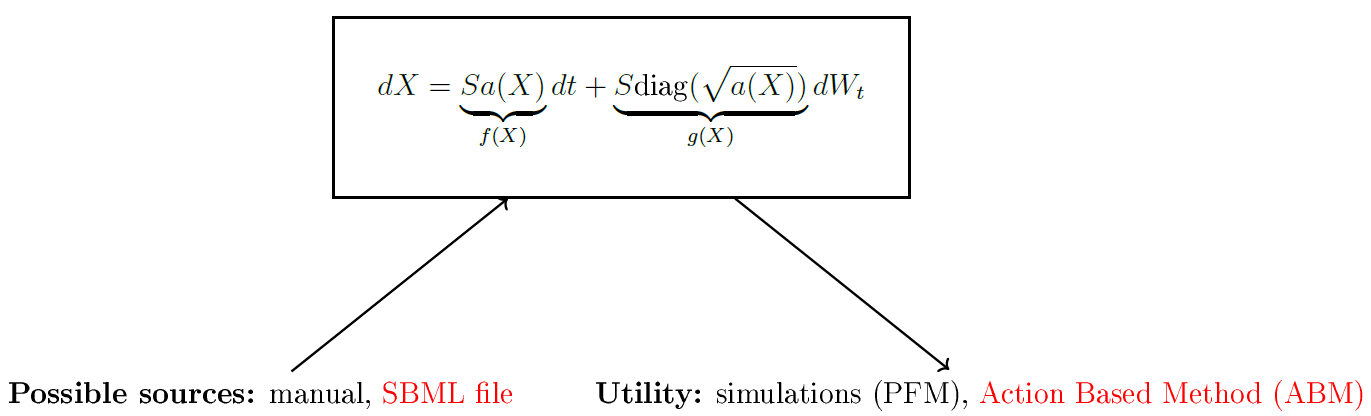
\includegraphics[width=\textwidth]{LT.PNG}
\end{figure}
\end{frame}

\begin{frame}{Possible sources: SBML file}
\begin{columns}
\begin{column}{0.5\textwidth}
   \begin{enumerate}
\item \textbf{General structure:} \\
\medskip
XML-based \\
Model object that inherits lists. \\
\bigskip
\item \textbf{Approach:} \\

\medskip
Strings --  metaprogramming $\rightarrow$ Julia ODEs. \\
Limited complexity (exceptions identifiable). \\
\end{enumerate}
\end{column}
\begin{column}{0.5\textwidth}  %%<--- here
    \begin{center}
     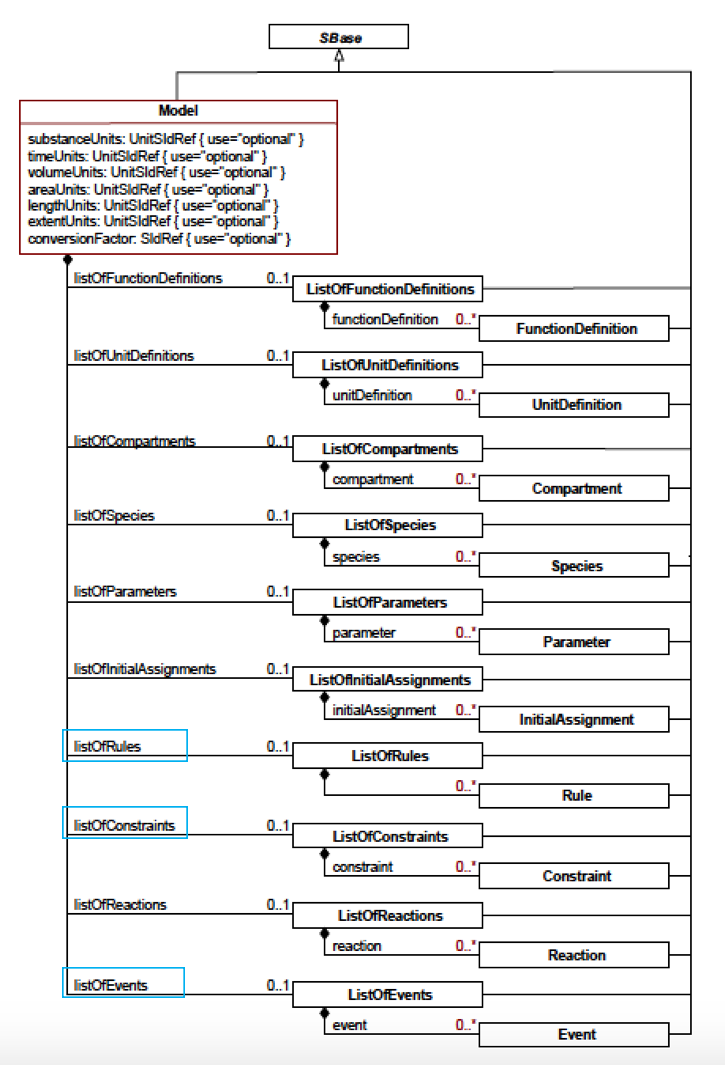
\includegraphics[width=0.8\textwidth]{Picture3.png}
     \end{center}
\end{column}
\end{columns}
\end{frame}

\begin{frame}{Possible sources: SBML file}
\begin{enumerate} 
\setcounter{enumi}{2}
\item \textbf{Validation:}
\end{enumerate}
\begin{figure}[h!]
\centering
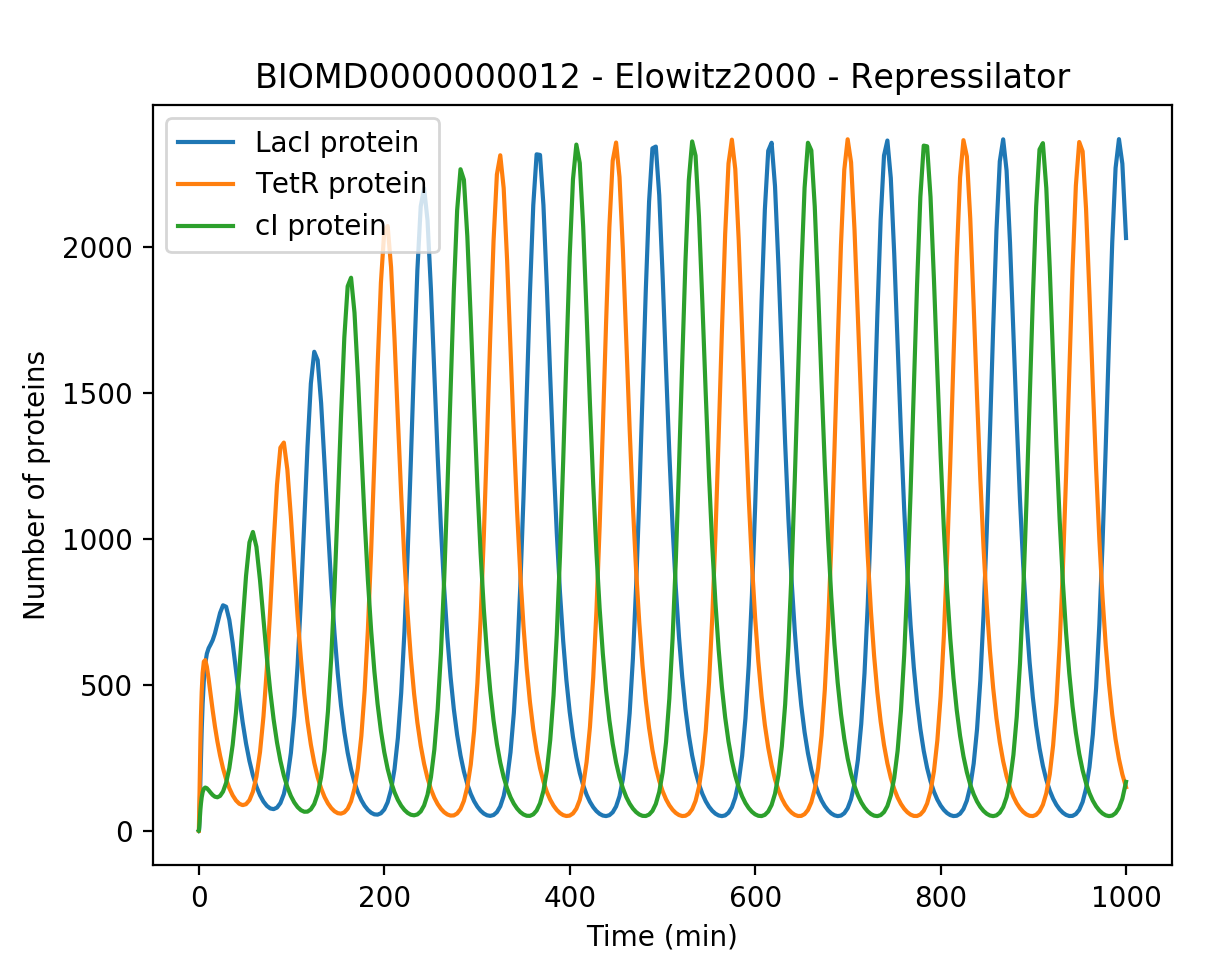
\includegraphics[width=0.40\textwidth]{BIOMD0000000012.png}
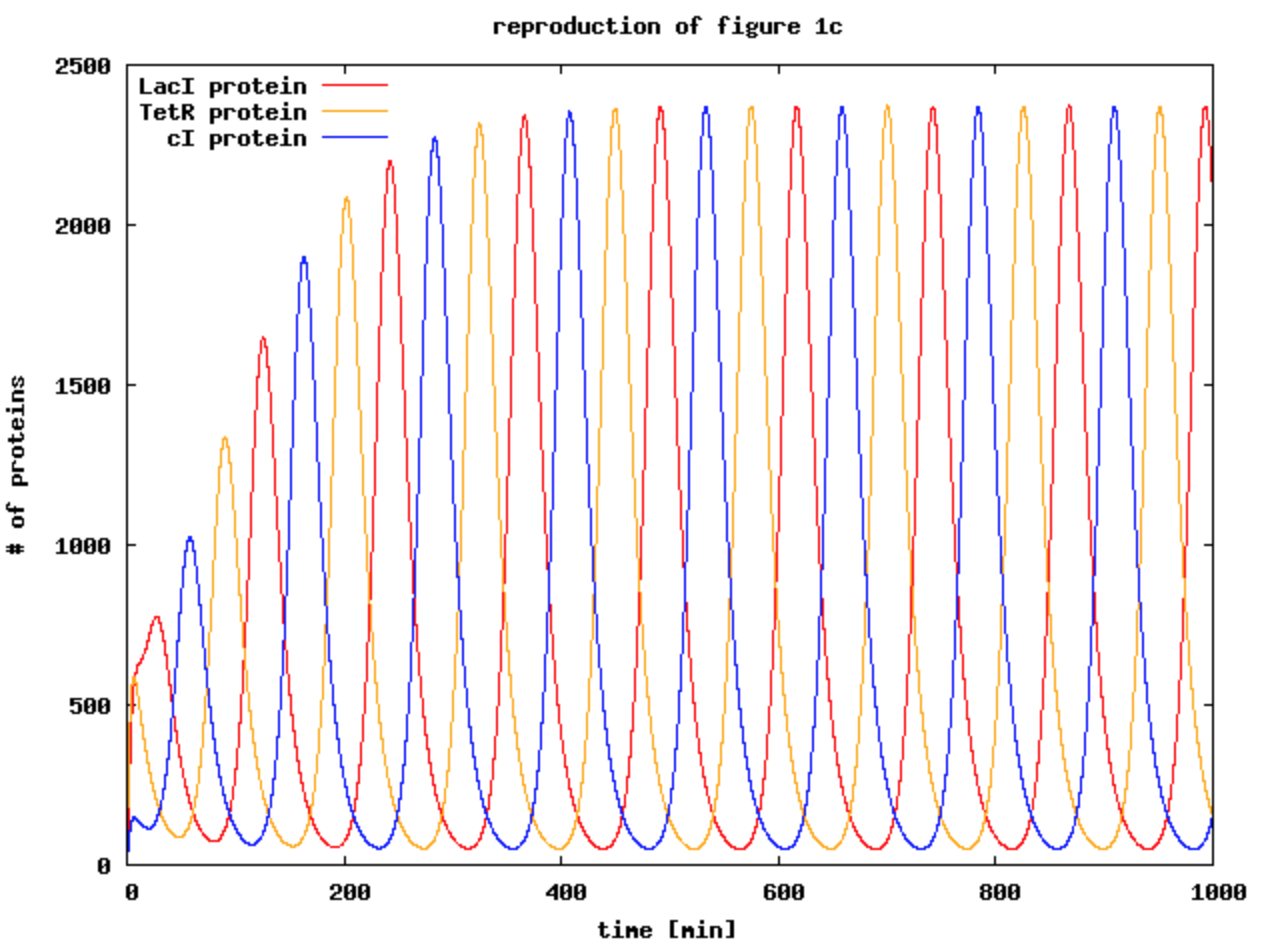
\includegraphics[width=0.40\textwidth]{Curated-BIOMD0000000012.png} \\
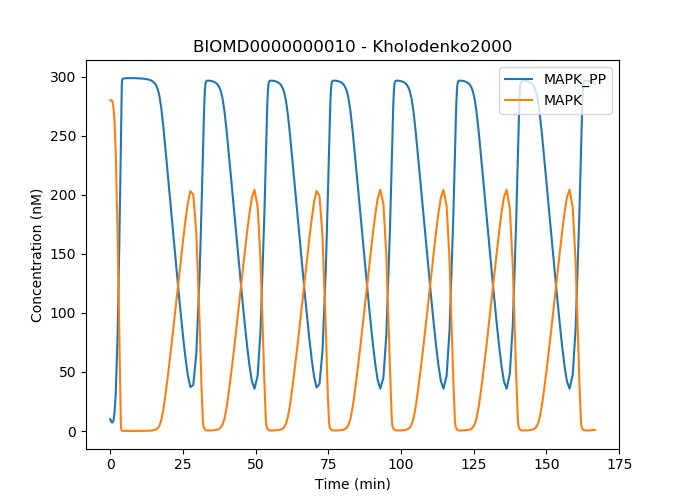
\includegraphics[width=0.40\textwidth]{BIOMD0000000010.png}
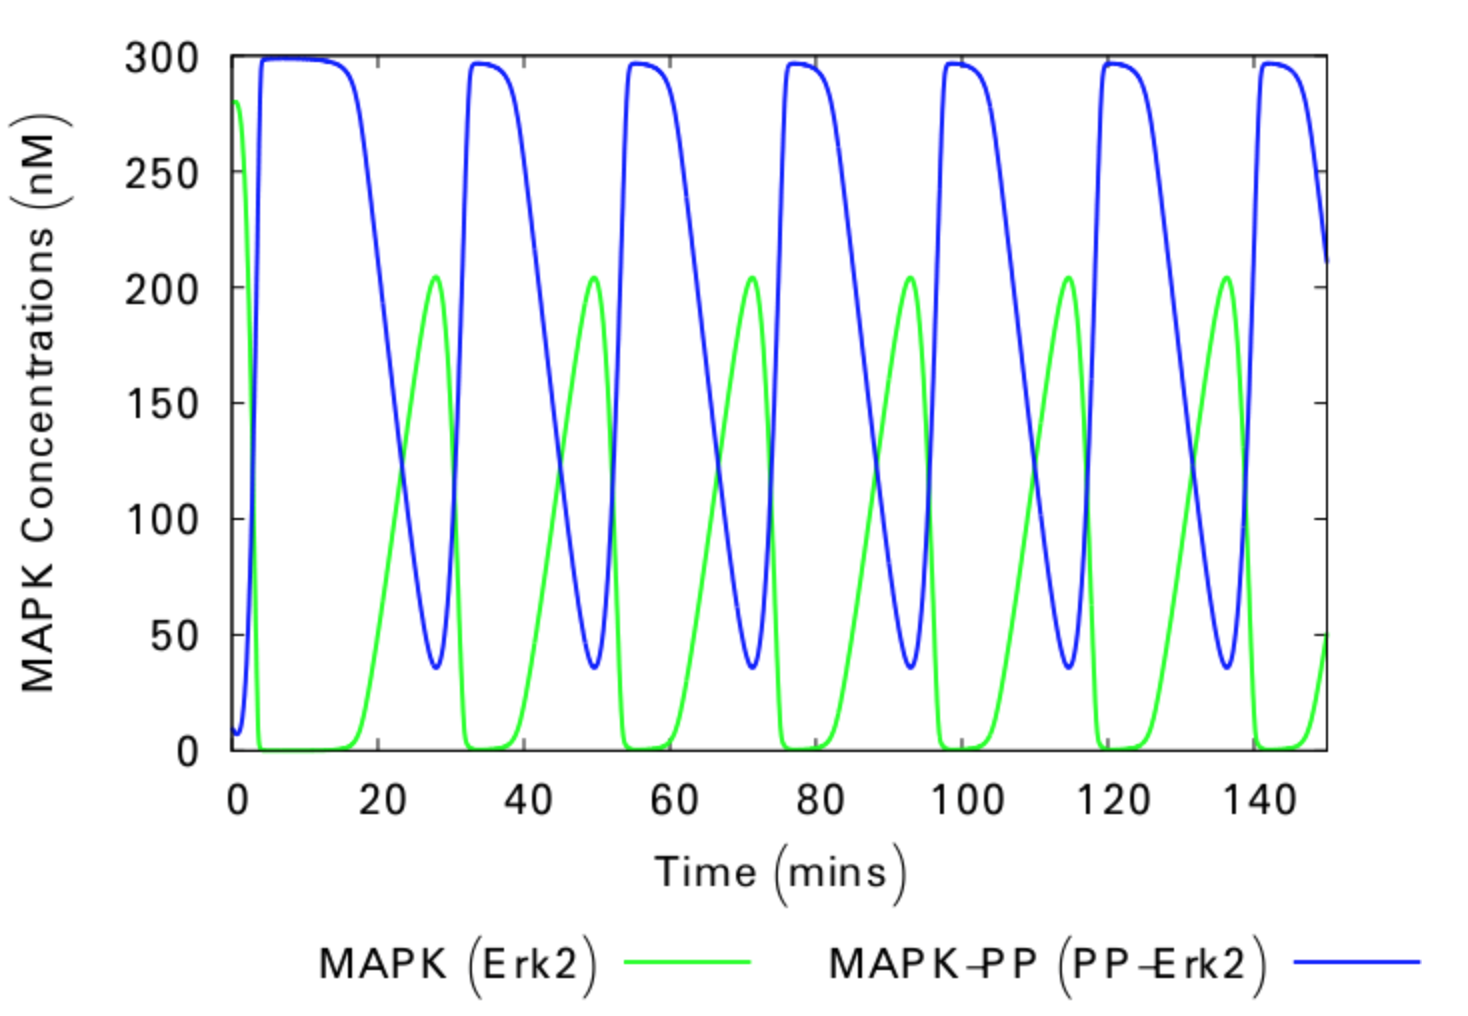
\includegraphics[width=0.40\textwidth]{Curated-BIOMD0000000010.png}
\end{figure}

\end{frame}

\begin{frame}{Utility: Action-Based Method (ABM)}
\textbf{Large deviations Theory:} \\
\bigskip
Action function: \\
\begin{equation}\label{action}
S(\varphi, T)=\int_{0}^{T}\sum_{i}(\dot{x}_{i}-f_{i}(x))^{2}/g_{i}^{2}(x) dt
\end{equation}

Quasi-potential barrier, $S$(minimum-action path): \\
\begin{equation}\label{MAP}
U(x_1, x_2) = \inf_{T>0} \inf_{\varphi \in \bar{{C}}_{x_1}^{x_2}(0,T)} S_T(\varphi)
\end{equation}

\begin{figure}[h!]
\centering
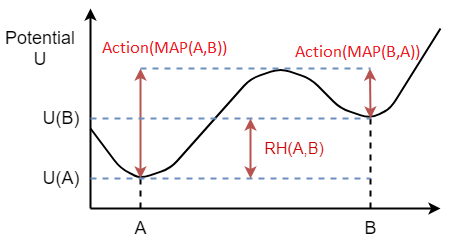
\includegraphics[width=0.45\textwidth]{RH.png}
\end{figure}
\end{frame}

\begin{frame}{Utility: Action-Based Method (ABM)}

Stability Analysis:
\begin{figure}[h!]
\centering
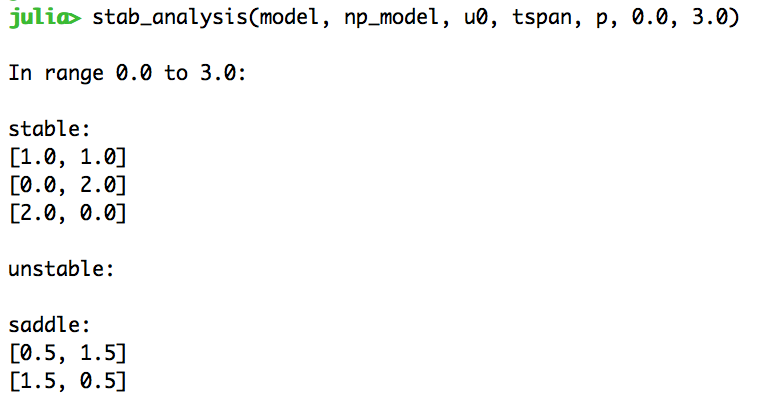
\includegraphics[width=0.40\textwidth]{stab-ex-2D.png}
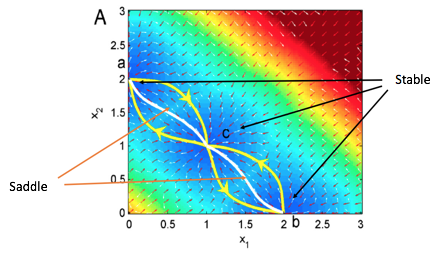
\includegraphics[width=0.35\textwidth]{stab-ex2.png}
\end{figure}

Genetic Algorithm:
\begin{figure}
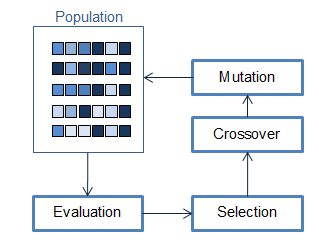
\includegraphics[width=0.35\textwidth]{genetic-algorithm-process.png} 
\end{figure}
\end{frame}

\section{Simulations, Probability Flux Method \& Kernel Density Estimation, 2D-Model Results [LD]}

\begin{frame}{Landscapes from Simulations of a SDE model}
\begin{figure}
\centering
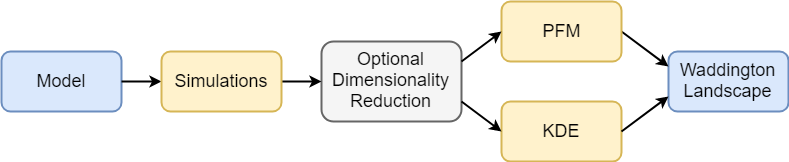
\includegraphics[width=1.0\textwidth]{PFMworkflow.png}
\caption{Workflow using simulations to build lanscapes}\label{pfmworkflow}
\end{figure}
\end{frame}
\begin{frame}{Simulations}
The analyzed model is a SDE:
\[ dX = f(X)dt + g(X)dW_{t}\]

From this model, using the DifferentialEquations package of Julia, the method runs simulations: 
\begin{itemize}
\item random initial points
\item fix amount of time
\end{itemize}

\begin{columns}
\begin{column}{0.35\textwidth}
\begin{figure}
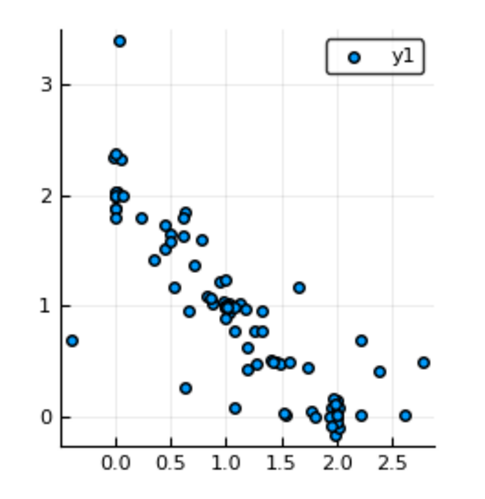
\includegraphics[width=\textwidth]{simplot.PNG}
\end{figure}
\end{column}
\begin{column}{0.65\textwidth}  %%<--- here
\begin{figure}
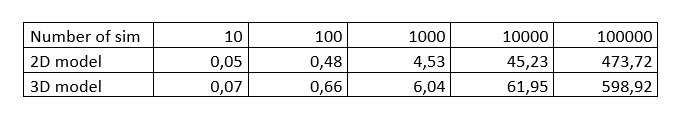
\includegraphics[width=\textwidth]{tabletimesim.PNG}
\end{figure}
\end{column}
\end{columns}
\end{frame}

\begin{frame}{Probability Flux Method}
The idea of the PFM is to compute the potential landscape $U$ thanks to:
\[ U \propto \ln (P_{s}) \]
where $P_{s}$ is the density function calculated from the simulations

We discretize the space and calculate the density distribution.
\begin{figure}
\centering
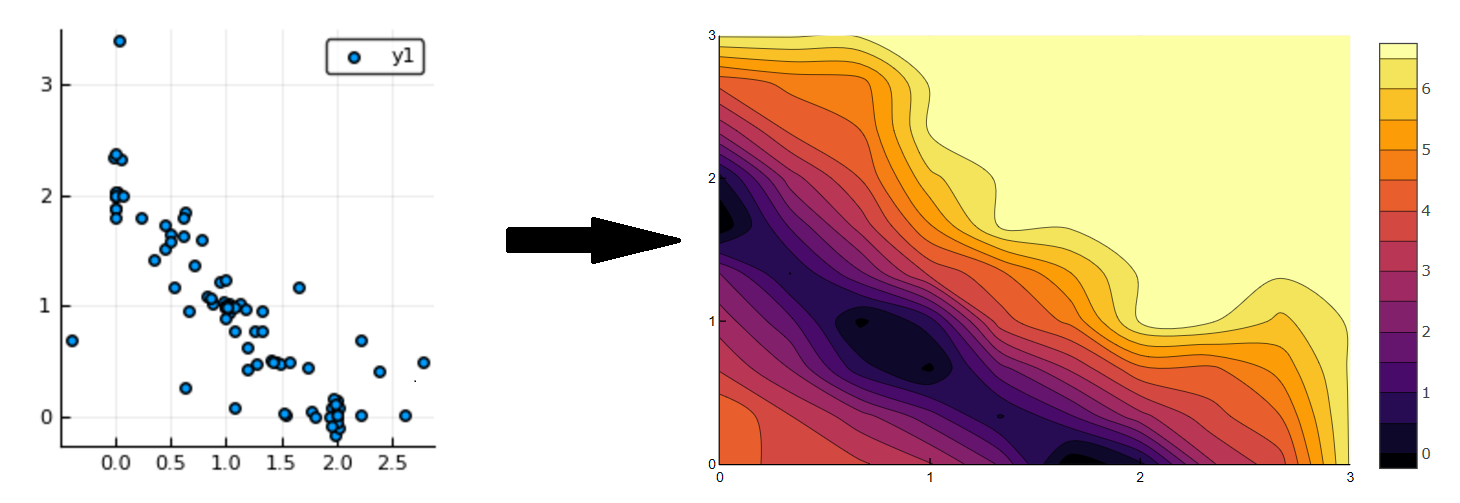
\includegraphics[width=0.80\textwidth]{simtoU.png}
\end{figure}

Main problems: Requires lot of simulations, does not describe well the low probability area of the space.
\end{frame}

\begin{frame}{Kernel Density Estimation}
KDE is a variant of the PFM where $P_{s}$ is calculated as a parameterized function $\hat{f_h}$ where $x_{i}$ are the results of the simulations and $h$ a bandwidth:
\[ \hat{f_h} (x) = \frac{1}{Nh} \sum_{i=1}^{N} K\left(\frac{x-x_i}{h}\right) \] Here $K$ is a kernel function, the Gaussian Kernel is the most widely used: \[ K(x) = \frac{1}{\sqrt{2\pi}} e ^ {- \frac{1}{2} x^2} \]

\begin{figure}
\centering
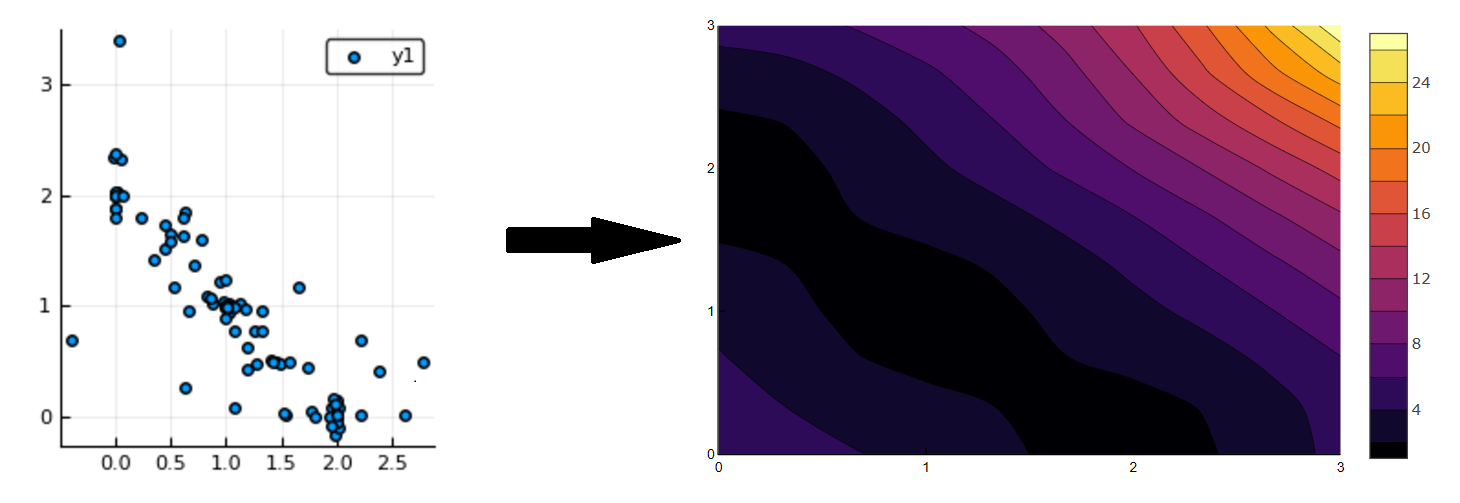
\includegraphics[width=0.61\textwidth]{simtoUkde.png}
\end{figure}
Main issue is the choice of the optimal bandwidth.
\end{frame}

\begin{frame}{Test on a 2D model}
The 2-dimensional model we use to test our methods is from a basic gene regulatory network of 2 nodes. These genes are self activating and mutually inhibiting each other.

\begin{figure}[!h]
\centering
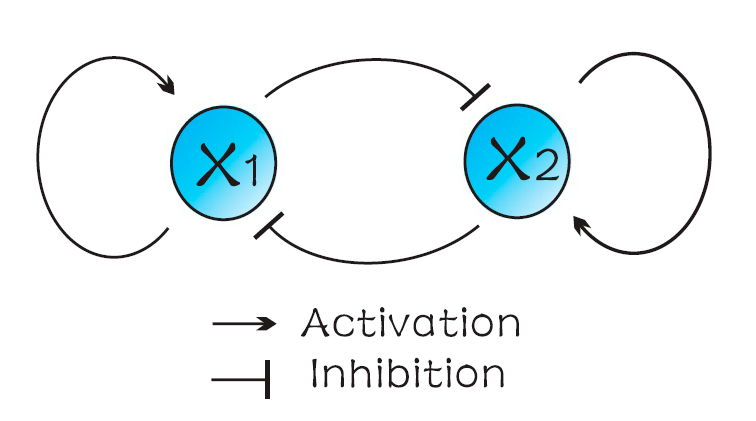
\includegraphics[width=0.4\textwidth]{2Dmodel.png}
\end{figure}
\small{
\[ dX_1= \left(\frac{a_1X_1^n}{S^n+X_1^n}+\frac{b_1S^n}{S^n+X_2^n} - k_1X_1\right)dt + \sqrt[]{\left|\frac{a_1X_1^n}{S^n+X_1^n}+\frac{b_1S^n}{S^n+X_2^n} - k_1X_1\right|} dW_t\]
\[ dX_2 = \left(\frac{a_2X_2^n}{S^n+x_2^n} +\frac{b_2S^n}{S^n+X_1^n} - k_2X_2\right)dt + \sqrt[]{\left|\frac{a_2X_2^n}{S^n+x_2^n} +\frac{b_2S^n}{S^n+X_1^n} - k_2X_2\right|} dW_t\]
}
\end{frame}

\begin{frame}{Results of the 2D model}
\begin{figure}[!h]
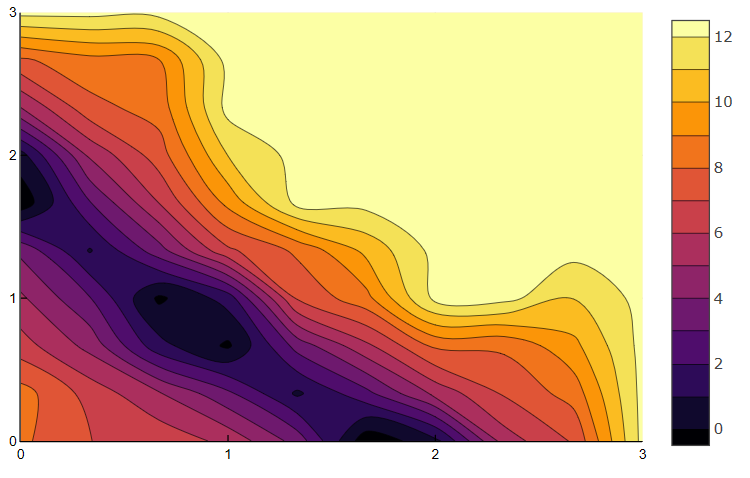
\includegraphics[width=0.33\textwidth]{pfm_prop_2Dmodel.PNG}
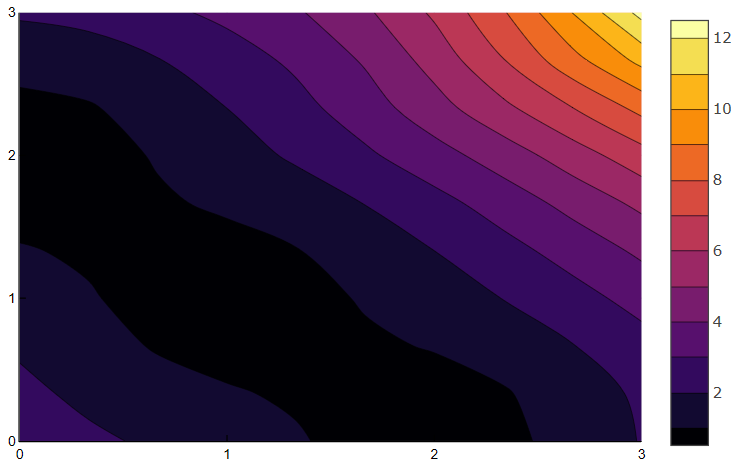
\includegraphics[width=0.33\textwidth]{kde_prop_2Dmodel.PNG}
\hspace{1.1cm}
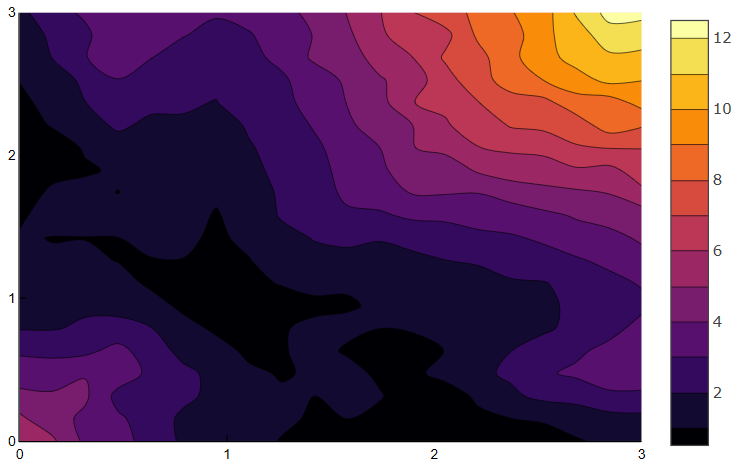
\includegraphics[width=0.33\textwidth]{abm_2Dmodel.PNG}
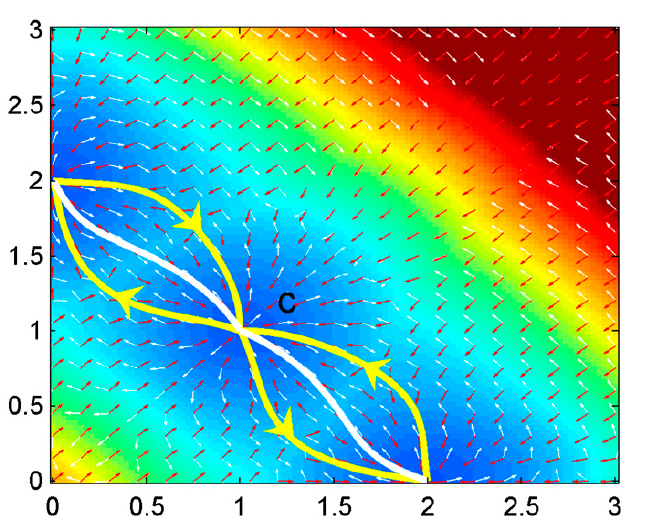
\includegraphics[width=0.33\textwidth]{control_2Dmodel.PNG}
\caption{Colored maps of the 2D model potential computed from PFM (top-left), PFM-KDE (top-right), ABM (bottom-left) and control plot (bottom-right). X1 in X-axis and X2 in Y-axis. }
\end{figure}
\end{frame}

\section{Data, Discussion \& Conclusion [MH]}

\begin{frame}{Landscapes from Data}
\begin{figure}
\centering
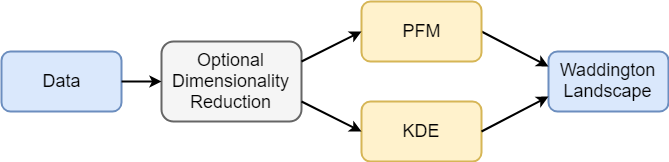
\includegraphics[width=0.8\textwidth]{MHworkflow.png}
\caption{Workflow using data to build landscapes}
\end{figure}
\begin{itemize}
\item Data points can be thought of as equivalent to end states from simulations of models
\item We apply the same approach to generate landscapes
\end{itemize}
\end{frame}


\begin{frame}{Landscapes from Data}

\begin{itemize}
\item 547 cells, 96 genes\footnote{Neil Smyth, University of Southampton}: seperated by time (0, 24, \ldots, 168 hours) or type (ESC, EPI, NPC)
\item Dimensionality Reduction: \begin{itemize}
\item Feature selection: highest correlation, information theory measures
\item Feature extraction: PCA, PPCA, etc. \\ \textcolor{red}{Loss of biological relevance}
\end{itemize}
$\Rightarrow$ 2 dimensions to generate landscape
\end{itemize}
\end{frame}


\begin{frame}{Landscapes from Data}
\begin{itemize}
\item Feature selection/extraction can determine the most informative landscapes
\item Common form of measurement noise in this type of data is false zeros
\end{itemize}
\begin{figure}
\centering
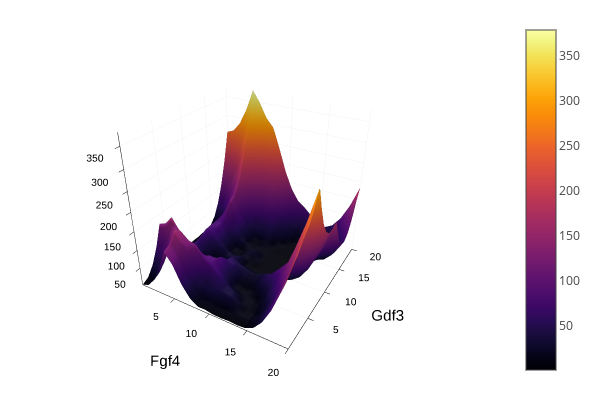
\includegraphics[width=0.33\textwidth]{Fgf4_Gdf3_data.png}
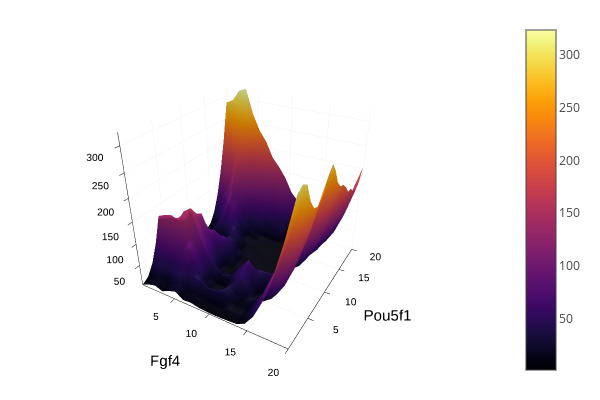
\includegraphics[width=0.33\textwidth]{Fgf4_Pou5f1_data.png}
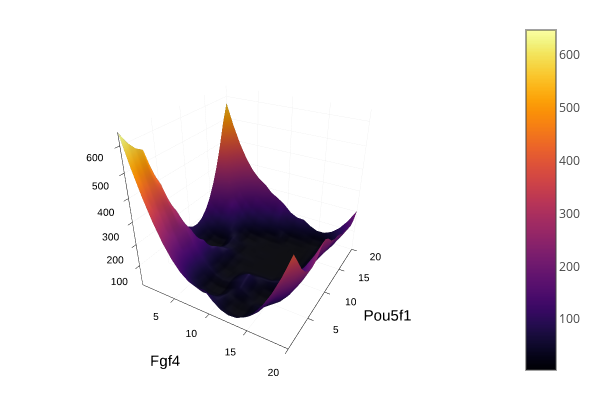
\includegraphics[width=0.33\textwidth]{Fgf4_Pou5f1_data_skipzeros.png}
\caption{Landscapes - highest correlation, highest MI, zeros removed.}
\end{figure}
\end{frame}

\begin{frame}{Landscapes from Data}
\begin{figure}
\centering
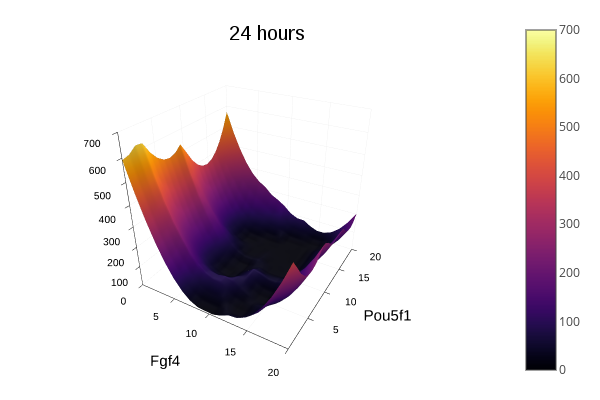
\includegraphics[width=0.4\textwidth]{Fgf4_Pou5f1_day1.png}
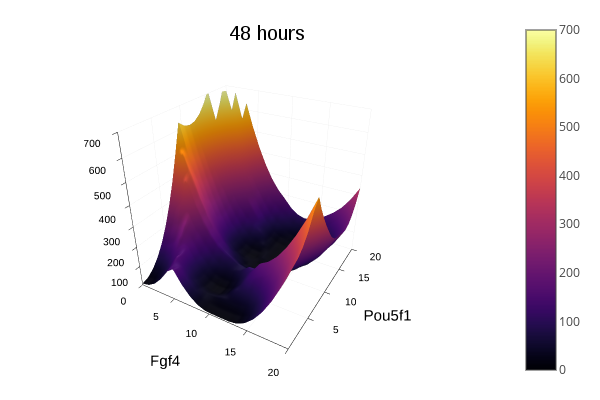
\includegraphics[width=0.4\textwidth]{Fgf4_Pou5f1_day2.png} \\
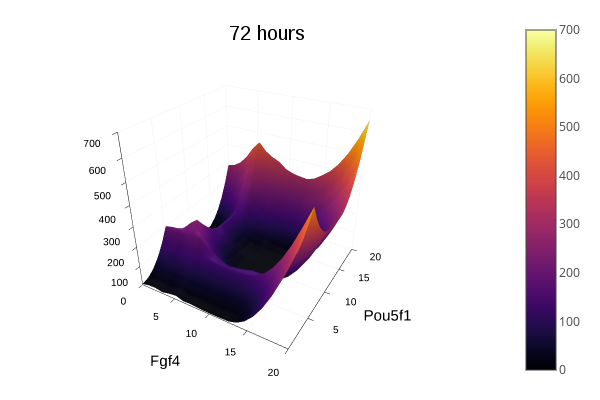
\includegraphics[width=0.4\textwidth]{Fgf4_Pou5f1_day3.png}
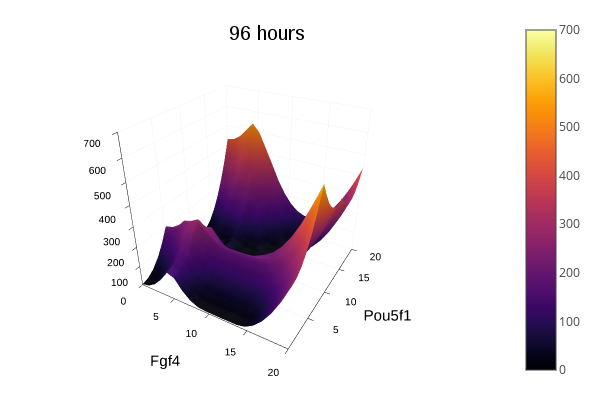
\includegraphics[width=0.4\textwidth]{Fgf4_Pou5f1_day4.png}
\caption{Separation of data by time allows visualisation of landscape evolution. Animations can be generated to show moving landscapes.}
\end{figure}
\end{frame}

\begin{frame}{Discussion}
\begin{itemize}
\item Julia: fast, clear mathematical syntax, growing availability of libraries (key to this project - DifferentialEquations, MultivariateStats, Plots), but still developing
\item Potential to develop techniques further to incorporate higher dimensional systems and datasets
\end{itemize}
\end{frame}

\begin{frame}{Summary}
\begin{itemize}
\item Developed tools to construct Waddington landscapes in Julia
\item Inputs: SBML file, model, data
\item Methods: ABM, PFM, KDE
\item Provide means for further exploration of landscapes, including stability analysis and dimensionality reduction
\end{itemize}
\end{frame}

\end{document}
